\section{Portability Across Workloads and Regions}\label{sec:results}
\subsection{Cross-Source Rankings}
\label{sec:cross-source-rankings}

Across the 3 source pairs $\times$ 6 operating regions (18 conditions),
Kendall's tau-b for the PRIMARY metric ranges from $0.55$ to $1.00$, with a
per-region mean between $0.69$ and $0.77$ (Figure~\ref{fig:portability-heatmap}). Every one of the 18 conditions has a
positive, non-trivial tau-b: comparative scheduler rankings are never
uncorrelated or inverted \emph{in aggregate} between any two sources at any
region. Portability is, however, visibly uneven across source \emph{pairs}
rather than uniform: Azure-2024 and Bailian/Qwen agree very strongly with
each other at every region ($\tau = 0.89$--$1.00$), while every
comparison involving BurstGPT is substantially lower ($\tau =
0.55$--$0.71$) -- a gap of roughly $0.2$--$0.4$ in Kendall's tau-b that
holds at all six regions, not just one. Top-1 agreement (the deterministic single top-choice policy) and top-3 agreement follow the same
source-pair pattern in the underlying evaluation data; we do not
tabulate top-1/top-3 separately in the main text to avoid restating the
same qualitative pattern three times, but the full table is part of the
preserved artifact (\S\ref{sec:artifact}).

\begin{figure}[h]
\centering
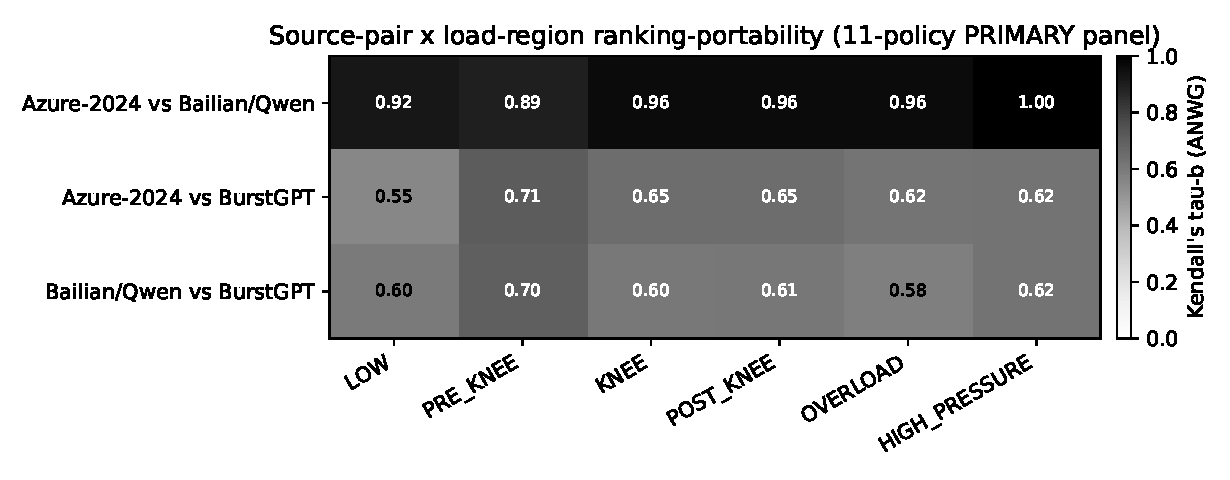
\includegraphics[width=0.85\textwidth]{figures/fig1_portability_heatmap.pdf}
\caption{Source-pair $\times$ load-region ranking-portability: Kendall's
tau-b between each pair of sources' PRIMARY-panel (11-policy) rankings on
the ANWG metric, at each of the six frozen operating regions
(\S\ref{sec:calibration}). Computed from the frozen ranking correlations artifact.}
\label{fig:portability-heatmap}
\Description{Heatmap of 18 historical simulator ANWG rank correlations. Azure--Bailian agreement is 0.89 to 1.00; comparisons involving BurstGPT are 0.55 to 0.71.}
\end{figure}

The min/max range in Figure~\ref{fig:portability-heatmap} makes clear that
portability is not homogeneous even within a region: the range at LOW
($0.55$--$0.92$) is nearly as wide as at any other region, and the range is
driven entirely by which source pair is compared, not by which region is
compared (\S\ref{sec:load-conditioning} tests region dependence
explicitly). No region shows uniformly low or uniformly high agreement
across all three source pairs simultaneously.

\subsection{Load Conditioning}
\label{sec:load-conditioning}

Load-level dependence is a secondary robustness/sensitivity analysis
(\S\ref{sec:rq}), reported here as a direct read of the same
\S\ref{sec:cross-source-rankings} table rather than a separate headline
claim of cross-source rank instability by itself. Secondary ranking statistics (Spearman's $\rho$ and top-1/top-3 overlap) exhibit an identical quantitative pattern and are omitted from the main tables for concision; their full values are preserved in the preserved analysis outputs. Figure~\ref{fig:portability-heatmap}'s
per-region mean tau-b is close to flat across the six regions ($0.69$ at
LOW, rising to $0.72$--$0.77$ elsewhere, no monotonic trend with load
factor); a leave-one-region-out comparison between the full six-region
grid and the four-region \texttt{LOW}/\texttt{PRE\_KNEE}/\texttt{KNEE}/
\texttt{OVERLOAD} subset used by \texttt{LOAD\_CALIBRATION\_SENSITIVITY}
(\S\ref{sec:robustness}) changes the mean tau-b by less than $0.01$
($0.728$ on the four-region subset versus $0.733$ on the full six-region
grid) -- the headline cross-source portability conclusion is not sensitive
to the choice of four-region versus six-region calibration grid. Load
regime does, however, materially affect \emph{where practically supported
reversals occur} (\S\ref{sec:reversals}): reversal counts are concentrated
at PRE\_KNEE and above, essentially absent at LOW.

\subsection{Pairwise Reversals}
\label{sec:reversals}

Of the 990 (policy pair) $\times$ (source pair, region) PRIMARY-metric
records (55 policy pairs among the 11 PRIMARY policies $\times$ 18
conditions), the
five-class breakdown (\S\ref{sec:uncertainty}) is: $906$
\texttt{STABLE\_NO\_SIGN\_CHANGE} ($91.5\%$), $48$
\texttt{MICROSCOPIC\_SIGN\_CHANGE} ($4.8\%$), $36$
\texttt{SUPPORTED\_PRACTICAL\_REVERSAL} ($3.6\%$), and zero records in
either \texttt{UNDEFINED\_UNESTIMABLE} or
\texttt{UNSUPPORTED\_SIGN\_CHANGE\_WIDE\_CI}. The large majority of
pairwise comparisons are stable; a small but non-trivial minority (about 1
in 28) are both practically and statistically supported reversals -- never
a majority, and never absent. The saved taxonomy contains no practical sign change with a wide interval. Microscopic changes are tested before the interval branch, so this is not evidence that practical and statistical criteria always agree.



Reversal counts are load-dependent: zero \texttt{SUPPORTED\_PRACTICAL\_REVERSAL}
records at \texttt{LOW}, rising to 6 at each of \texttt{PRE\_KNEE},
\texttt{KNEE}, and \texttt{POST\_KNEE}, 10 at \texttt{OVERLOAD}, and 8 at
\texttt{HIGH\_PRESSURE} (Table~\ref{tab:region-counts}). All 36 involve BurstGPT, but they span five policy pairs: SLAI--vLLM
(10), Sarathi--SLAI (9), chunked-vLLM--SLAI (9), Sarathi--vLLM (4), and
chunked-vLLM--vLLM (4), where these names abbreviate historical simulator
identifiers. Earlier manuscript wording attributing all 36 records to one
pair was incorrect. The single largest-effect-size supported reversal (operationalized
as the smaller-magnitude of the two conditions' practical margins, the
binding constraint under the frozen practical-margin rule,
\S\ref{sec:uncertainty}) is \texttt{slai\_faithful} vs.\
\texttt{vllm\_faithful} at \texttt{HIGH\_PRESSURE}, comparing Azure-2024
(or, at an effectively tied effect size, Bailian/Qwen) against BurstGPT --
this is the case selected for the historical physical comparison under the frozen
selection rule (\S\ref{sec:real-system}).

A representative stable comparison, used as a null-result control alongside
the reversal case in the historical physical design
(\S\ref{sec:real-system}), is the source pair with both the highest tau-b
and (among the highest-tau conditions) the narrowest bootstrap interval:
Azure-2024 vs.\ Bailian/Qwen at \texttt{HIGH\_PRESSURE} ($\tau = 1.00$,
95\% CI $[0.90, 1.00]$).

\subsection{Temporal Portability}
\label{sec:temporal}

Following the frozen temporal design (\S\ref{sec:temporal-design}), four
temporal record types are reported separately, each under its source's own
chronology, and never merged into a single ``temporal/domain OOD'' number:
BurstGPT's EARLY/MIDDLE/LATE tercile split (primary) and EARLY/LATE bisect
(sensitivity check on the tercile boundary), Azure-2024's absolute calendar
split, and Bailian/Qwen's \texttt{RELATIVE\_CHRONOLOGY\_ONLY} comparison,
for which no calendar-based claim is made. All values are keyed identically
to the source temporal robustness artifact. The canonical results reveal high rank stability across time: BurstGPT's tercile split shows strong agreement between EARLY and LATE chunks across non-LOW load regions ($\tau_b \in [0.81, 1.0]$), while the BISECT sensitivity check yields similarly stable correlations ($\tau_b \in [0.72, 0.80]$). At LOW, one BurstGPT tercile comparison instead has $\tau_b=-0.10$; this exception must not be hidden by a non-LOW summary. Azure's calendar split produces near-perfect correlation ($\tau_b \in [0.90, 1.0]$), and Bailian's relative-chronology split likewise exhibits minimal rank change ($\tau_b \in [0.94, 1.0]$).

Although the frozen protocol for this research question specified an analysis of temporal, provider, and domain shifts, a standalone domain-shift component was not separately operationalized in the final artifacts. The evidence reported here addresses the temporal component directly. The frozen cross-source comparisons (\S\ref{sec:cross-source-rankings}) include the one genuine provider boundary in this corpus (Bailian/Qwen on Alibaba Cloud versus the two Microsoft-infrastructure sources, \S\ref{sec:sources}), but the design does not isolate a causal provider effect from ordinary cross-source variation -- BurstGPT-vs-Azure is a cross-source, not cross-provider, comparison; domain shift, like the provider component, is addressed only implicitly through these same cross-source comparisons and was not separately operationalized.

\subsection{Point estimates and saved uncertainty}
\begin{table}[t]\centering
\caption{All 18 primary source-pair comparisons. A=Azure, B=Bailian,
G=BurstGPT. Intervals are the preserved 95\% window-bootstrap intervals;
M1 independently reproduced the point estimates but did not rerun intervals.}
\label{tab:all-correlations}
\begin{tabular}{llrr}\toprule
Region & Pair & Tau-b & Saved 95\% interval\\\midrule
LOW & A--B & 0.920 & [0.864, 0.920]\\
LOW & A--G & 0.551 & [0.203, 0.551]\\
LOW & B--G & 0.599 & [0.220, 0.599]\\
PRE\_KNEE & A--B & 0.893 & [0.893, 1.000]\\
PRE\_KNEE & A--G & 0.709 & [0.450, 0.753]\\
PRE\_KNEE & B--G & 0.697 & [0.404, 0.753]\\
KNEE & A--B & 0.958 & [0.914, 1.000]\\
KNEE & A--G & 0.646 & [0.578, 0.729]\\
KNEE & B--G & 0.604 & [0.521, 0.688]\\
POST\_KNEE & A--B & 0.958 & [0.958, 1.000]\\
POST\_KNEE & A--G & 0.647 & [0.510, 0.678]\\
POST\_KNEE & B--G & 0.606 & [0.469, 0.647]\\
OVERLOAD & A--B & 0.958 & [0.958, 1.000]\\
OVERLOAD & A--G & 0.620 & [0.566, 0.620]\\
OVERLOAD & B--G & 0.580 & [0.525, 0.620]\\
HIGH\_PRESSURE & A--B & 1.000 & [0.904, 1.000]\\
HIGH\_PRESSURE & A--G & 0.623 & [0.550, 0.712]\\
HIGH\_PRESSURE & B--G & 0.623 & [0.550, 0.699]\\
\bottomrule\end{tabular}\end{table}
The intervals describe a window-resampling procedure on the sampled
sources, not uncertainty over hardware architectures or all production
populations. Their width is distinct from between-source variation in
point estimates. Reporting them next to the full comparison set avoids
selecting only the strongest or weakest agreement. Stable source pairs
and the absence of a supported reversal at LOW remain part of the result.
